\documentclass[12pt]{article}

\usepackage[margin=1in]{geometry}
\usepackage{graphicx}
\usepackage{longtable}
\usepackage{booktabs}
\usepackage{hyperref}
\usepackage{float}
\usepackage{array}
\usepackage{xcolor}

\hypersetup{
  colorlinks=true,
  linkcolor=black,
  urlcolor=blue,
  pdftitle={Incident Response Report - IR-2026-001},
  pdfauthor={Sentinel Ridge Cybersecurity}
}

% Convenience column type for wrapped table cells
\newcolumntype{L}[1]{>{\raggedright\arraybackslash}p{#1}}

\newcommand{\ptext}[1]{\textcolor{red}{[#1]}}

\graphicspath{{./}{capturas/}}

\begin{document}

%============================ COVER PAGE ============================
\begin{titlepage}
\centering
\vspace*{0.5cm}


\includegraphics[width=0.45\textwidth]{logo.png}\\[2cm]

{\Huge\bfseries Incident Response Report}\\[0.6cm]
{\LARGE Workstation Compromise via Drive-By\\Exploit Kit and Xtreme RAT}\\[2cm]

\begin{tabular}{rl}
\textbf{Affected Organization:} & Northbridge Financial Services\\[4pt]
\textbf{Incident Number:} & IR-2026-001\\[4pt]
\textbf{Date Published:} & 2026-07-01\\[4pt]
\textbf{Prepared By:} & Havi Arji\\[4pt]
\textbf{Course:} & CYBR 445\\[4pt]
\textbf{Instructor:} & Alex Hepp\\[4pt]
\textbf{Investigation Performed By:} & 4rji Cybersec \\[4pt]
\textbf{Classification:} & Privileged and Confidential\\
\end{tabular}

\vfill

\begin{figure}[H]
\centering
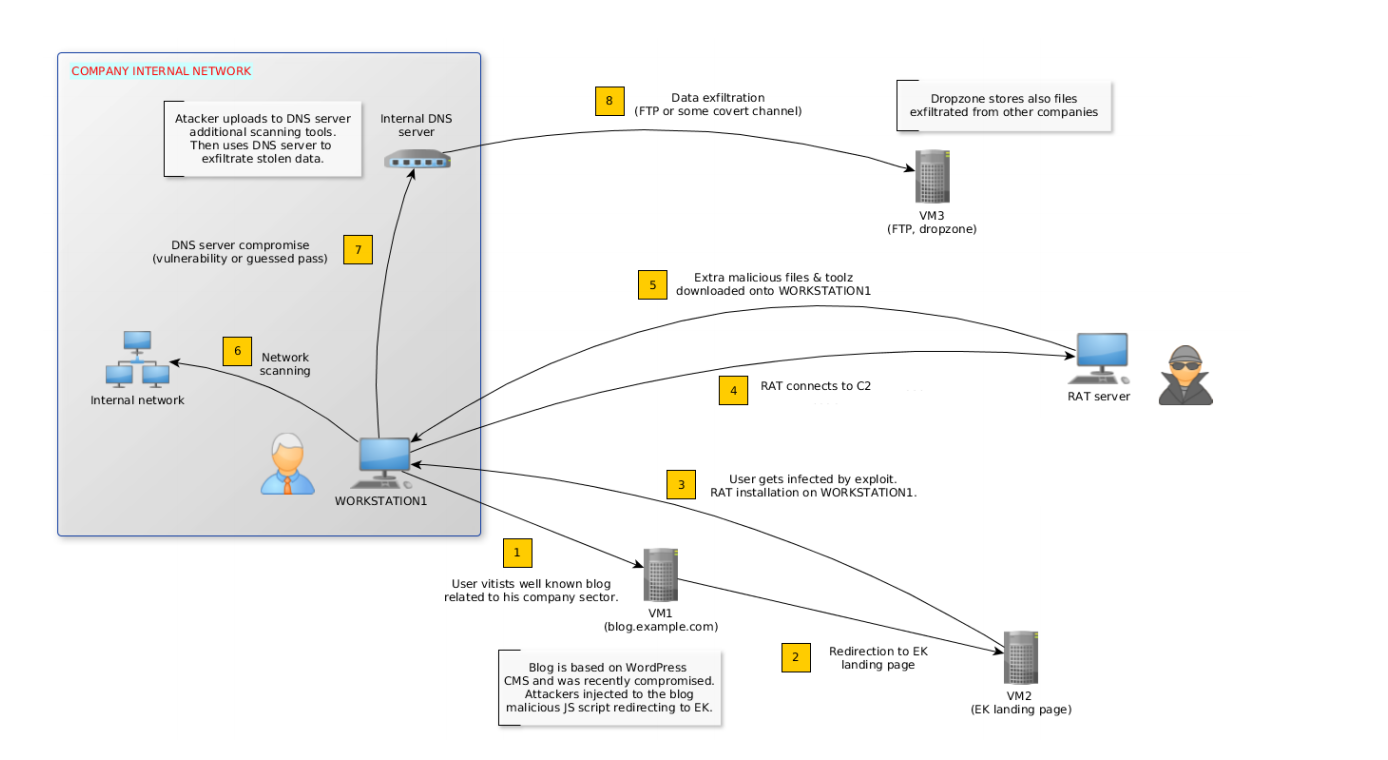
\includegraphics[width=0.9\textwidth]{fig-01.png}
\caption*{High-level attack diagram: infection via Exploit Kit, RAT installation, internal scanning, and exfiltration.}
\end{figure}

\end{titlepage}

\tableofcontents
\newpage

%============================ 1. EXEC SUMMARY ============================
\section{Executive Summary}

Northbridge Financial Services engaged Sentinel Ridge Cybersecurity to investigate the compromise of an employee Windows workstation. The incident was discovered after security staff noticed anomalous behavior on the host and captured a live memory image and a full forensic disk image for analysis. The engagement was sponsored by Northbridge Financial Services' executive leadership team.

The investigation determined that the workstation was infected with \textbf{Xtreme RAT}, a commodity remote-access trojan that gives an attacker full remote control of a victim machine. The infection began when the user browsed to a legitimate but compromised website (\texttt{blog.mycompany.ex}). That site had been tampered with to silently redirect the browser to an \textbf{Exploit Kit} hosted at \texttt{blog.mysportclub.ex}. Because the workstation ran an outdated web browser and browser plugin, the Exploit Kit succeeded in running code without any user interaction beyond visiting the page --- a ``drive-by'' attack. The malware installed itself, established persistence so it would survive reboots, and then downloaded a toolkit of hacking utilities. Over the following two hours the attacker profiled the machine, scanned the internal network, attempted to guess passwords for other systems, connected to at least one internal host, and transferred data using file-copy tools --- behavior consistent with an active, hands-on-keyboard intruder attempting to move deeper into the network.

The response goal was to establish how the machine was compromised, what the attacker did, which systems and accounts were affected, and which indicators the organization should hunt for enterprise-wide. Based on the evidence, the affected workstation was isolated and reimaged, associated accounts were reset, malicious files and persistence were removed, and the attacker's infrastructure was blocked. The forensic activity captured in the evidence spans \textbf{2016-08-16 12:54 UTC (system boot) to approximately 14:50 UTC (last observed attacker tool execution)}.

%============================ 2. TIMELINE ============================
\section{Timeline}

All times are UTC. The host clock was configured for UTC+2 (local time = UTC + 2 hours), as confirmed by registry evidence (13:03:10 UTC = 15:03:10 local).

\begin{longtable}{L{2.6cm} L{7.5cm} L{4.2cm}}
\toprule
\textbf{Date/Time (UTC)} & \textbf{Event} & \textbf{Source of Evidence}\\
\midrule
\endhead
2016-08-16 12:54:24 & Workstation booted & Volatility \texttt{pslist}\\
2016-08-16 13:02:46 & User browses to compromised site \texttt{blog.mycompany.ex} & Firefox history\\
2016-08-16 13:02:57 & \texttt{svchost.exe} (Xtreme RAT) created in \texttt{\%TEMP\%}; \texttt{Run}/\texttt{RunOnce} keys modified & Filesystem; RegRipper \texttt{regtime}\\
2016-08-16 13:03:03--13:03:04 & \texttt{update.exe} (Xtreme RAT) executed & Prefetch; \texttt{pslist}\\
2016-08-16 13:03:10 & Persistence subkey \texttt{GhCtxq8t} created; \texttt{update.exe} first execution & RegRipper / WRR\\
2016-08-16 13:03:16 & Firefox crash report tied to Flash plugin & Application logs\\
2016-08-16 13:07:36 & \texttt{update.exe} spawns first \texttt{cmd.exe}; \texttt{whoami}/\texttt{ipconfig} 13:08--13:10 & \texttt{pslist}; Prefetch\\
2016-08-16 13:10:03 / 13:10:13 & \texttt{54948tp.exe} created and executed (downloads toolkit) & Filesystem; Prefetch\\
2016-08-16 13:14:47 & \texttt{EpUpdate} toolkit directory created; mimikatz \& BPD run 13:14:48 & Filesystem; Prefetch\\
2016-08-16 13:34:25--13:34:51 & Batch of local system-profiling commands; \texttt{sysinfo.txt} written & Prefetch; SystemProfile\\
2016-08-16 $\sim$13:56--13:59:36 & Nmap scans of 192.168.5.1, .10, .15 & Prefetch; \texttt{netscan/} XML\\
2016-08-16 14:02:04--14:04:43 & Event ID 4798 enumeration; Hydra executed 14:04:44 & Windows Event Log; Prefetch\\
2016-08-16 14:10:49--14:23:31 & \texttt{plink.exe} run six times; PuTTY \texttt{SSHHostKeys} for 192.168.5.10 written 14:11:26 & Prefetch; RegRipper / WRR\\
2016-08-16 14:47:12--14:50:09 & \texttt{pscp.exe} executed three times (data transfer) & Prefetch\\
\bottomrule
\end{longtable}

%============================ 3. FINDINGS ============================
\section{Findings}

An employee workstation belonging to Northbridge Financial Services was fully compromised by an attacker using the \textbf{Xtreme RAT} remote-access trojan. The compromise was not the result of the employee downloading an obviously malicious file; instead, the user simply visited a trusted website that had been secretly modified by attackers. That website redirected the browser, in the background, to an \textbf{Exploit Kit} that took advantage of outdated software on the workstation (Mozilla Firefox 33.0.3 and Adobe Flash 18.0.0.194) to install malware automatically. This is a classic drive-by compromise and highlights the risk of running unpatched browser software.

Once installed, the malware made itself persistent so it would run every time the user logged in, and it downloaded a full attacker toolkit including credential-stealing tools (mimikatz, a browser-password dumper, Pwdump), a network scanner (Nmap), a password-guessing tool (THC Hydra), and remote-access/file-transfer tools (plink and pscp from PuTTY). Evidence shows the attacker used these tools in a logical progression: they first learned about the machine and the internal network, scanned three internal hosts (192.168.5.1, 192.168.5.10, 192.168.5.15), attempted to crack passwords, connected to internal host 192.168.5.10, and then ran file-transfer tools consistent with moving data in or out of the environment.

The affected workstation and the user account that was logged in at the time are considered compromised, and internal host 192.168.5.10 is a strong candidate for follow-on compromise and requires its own examination. The strongest indicators for enterprise-wide hunting are the malicious file paths (\texttt{\%APPDATA\%\textbackslash HostData\textbackslash update.exe}, \texttt{\%TEMP\%\textbackslash svchost.exe}, \texttt{\%APPDATA\%\textbackslash EpUpdate\textbackslash}), the persistence registry key \texttt{GhCtxq8t}, the attacker domains \texttt{blog.mycompany.ex} and \texttt{blog.mysportclub.ex}, and the associated IP address 151.80.137.2. Evidence used included a memory image, a full disk image, Prefetch files, Windows Event Logs, and registry hives. In response, the workstation was isolated and reimaged, affected credentials were reset, the WDigest cleartext-credential change was reverted, persistence and malicious files were removed, and attacker infrastructure was blocked at the perimeter.

%============================ 4. INVESTIGATIVE QUESTIONS ============================
\section{Investigative Questions}

\subsection*{Question 1: How was the workstation initially compromised?}
\textbf{Answer:} Through a drive-by download. The user visited \texttt{blog.mycompany.ex}, a legitimate site injected with a hidden \texttt{<iframe>} pointing to an Exploit Kit at \url{http://blog.mysportclub.ex/wp-content/uploads/hk/task/opspy/index.php}. The kit served multiple exploits targeting the outdated browser and Flash plugin, one of which downloaded and executed the initial payload.\\
\textbf{Supporting Evidence:} Firefox history (visit at 13:02:46); cached \texttt{blog.mycompany.ex.htm} with the iframe injection; Exploit-Kit download pattern from \texttt{blog.mysportclub.ex}; Flash-related Firefox crash at 13:03:16 (Figures 17--22).

\subsection*{Question 2: What malware was installed, and where does it live on disk?}
\textbf{Answer:} \textbf{Xtreme RAT}. Its code was found in memory in three processes (\texttt{svchost.exe} PID 4888, \texttt{explorer.exe} PID 4872, \texttt{update.exe} PID 5172) and confirmed on disk by ClamAV. The primary persistent copy is \texttt{\%APPDATA\%\textbackslash HostData\textbackslash update.exe}, with a copy at \texttt{\%TEMP\%\textbackslash svchost.exe}.\\
\textbf{Supporting Evidence:} Volatility \texttt{yarascan} hits (Xtreme/xtreme\_rat/xtremrat); UPX-packing overlap; ClamAV confirmation (Figures 5--7, 16).

\subsection*{Question 3: Did the attacker establish persistence?}
\textbf{Answer:} Yes. At 13:02:57 the \texttt{Run}/\texttt{RunOnce} subkeys were modified, and at 13:03:10 a subkey \texttt{GhCtxq8t} was created. WRR analysis linked \texttt{GhCtxq8t} to \texttt{update.exe}; its \texttt{FirstExecution} value confirms \texttt{update.exe} first ran at 13:03:10 UTC (15:03:10 local), ensuring restart at logon.\\
\textbf{Supporting Evidence:} RegRipper \texttt{regtime} timeline and WRR inspection of \texttt{NTUSER.DAT} (Figures 34--35).

\subsection*{Question 4: What tools did the attacker deploy, and how did they arrive?}
\textbf{Answer:} A downloader, \texttt{54948tp.exe} (py2exe), created at 13:10:03 and executed at 13:10:13, fetched \texttt{data\_32.bin} from \url{http://blog.mysportclub.ex/wp-content/uploads/hk/files/data_32.bin}, decrypted and unpacked it into \texttt{\%APPDATA\%\textbackslash EpUpdate\textbackslash}. That directory held mimikatz, BrowserPasswordDump, NirCmd, Nmap, Pwdump, plink/pscp, THC Hydra, a \texttt{passwords.txt} wordlist, and \texttt{wdigest.reg} (enables \texttt{UseLogonCredential}).\\
\textbf{Supporting Evidence:} Decompiled \texttt{54948tp.exe}/\texttt{3568226350.exe} (\texttt{DOWNLOAD\_URL}, \texttt{get\_toolz}); \texttt{EpUpdate} created 13:14:47; Prefetch mimikatz/BPD at 13:14:48 (Figures 23--24, 29).

\subsection*{Question 5: Was there internal reconnaissance, lateral movement, or exfiltration?}
\textbf{Answer:} Yes to all three. The attacker profiled the system (13:34:25--13:34:51, plus earlier \texttt{whoami}/\texttt{ipconfig}), scanned three internal hosts with Nmap 7.12 around 13:56--13:59, ran THC Hydra at 14:04:44 (correlated with Event 4798 at 14:02--14:04), executed \texttt{plink.exe} six times (14:10:49--14:23:31) and \texttt{pscp.exe} three times (14:47:12--14:50:09). A PuTTY \texttt{SSHHostKeys} entry for 192.168.5.10 (14:11:26) indicates an SSH connection to that host.\\
\textbf{Supporting Evidence:} Prefetch; \texttt{netscan/} Nmap XML; Event 4798; RegRipper PuTTY \texttt{SSHHostKeys} (Figures 26, 30--33, 36--37).

\subsection*{Question 6: What vulnerabilities enabled the exploit, and which IOCs should be hunted?}
\textbf{Answer:} The host ran outdated \textbf{Firefox 33.0.3} and \textbf{Adobe Flash 18.0.0.194}; kit code referenced multiple exploits including \textbf{CVE-2012-3993}. Enterprise-wide, hunt the paths \texttt{\%APPDATA\%\textbackslash HostData\textbackslash update.exe}, \texttt{\%TEMP\%\textbackslash svchost.exe}, \texttt{\%APPDATA\%\textbackslash EpUpdate\textbackslash}; the key \texttt{GhCtxq8t}; domains \texttt{blog.mycompany.ex} and \texttt{blog.mysportclub.ex}; IP 151.80.137.2; and filenames \texttt{update.exe}, \texttt{54948tp.exe}, \texttt{3568226350.exe}.\\
\textbf{Supporting Evidence:} Registry Uninstall data; ClamAV detection of CVE-2012-3993 exploit code; IOC table (Figures 38--40).

\clearpage
%============================ 5. SYSTEMS / PEOPLE ============================
\section{Systems / People Involved}

\begin{longtable}{L{3.0cm} L{2.2cm} L{3.4cm} L{2.8cm} L{2.4cm}}
\toprule
\textbf{Hostname / Person} & \textbf{IP Address} & \textbf{Role / Purpose} & \textbf{Pertinent Evidence (UTC)} & \textbf{Compromise Found}\\
\midrule
\endhead
Affected workstation (hostname not identified) & Not identified & User endpoint; source of memory and disk images & 2016-08-16 12:54--14:50 & Yes --- Xtreme RAT, persistence, tooling\\
Logged-in user account (username not identified) & N/A & Interactive user; \texttt{NTUSER.DAT} modified for persistence & 2016-08-16 13:02:57+ & Yes --- session used for persistence \& tools\\
Internal host & 192.168.5.10 & Targeted by Nmap and SSH (plink) & 13:59 / 14:11:26 & Suspected --- SSH key recorded\\
Internal host & 192.168.5.1 & Scanned (likely gateway) & $\sim$13:59 & Scanned only\\
Internal host & 192.168.5.15 & Scanned & $\sim$13:59 & Scanned only\\
Attacker infrastructure & 151.80.137.2 & Resolution of \texttt{blog.mycompany.ex} & Day of investigation & N/A --- external\\
Attacker infrastructure (\texttt{blog.mysportclub.ex}) & Not identified & Exploit Kit / payload host & 13:02--13:10 & N/A --- external\\
\bottomrule
\end{longtable}

%============================ 6. IOCs ============================
\section{Indicators of Compromise}

\begin{longtable}{c L{2.4cm} L{4.0cm} L{3.2cm} L{3.0cm}}
\toprule
\textbf{\#} & \textbf{IOC Type} & \textbf{IOC Value} & \textbf{Why It Matters} & \textbf{Enterprise Search}\\
\midrule
\endhead
1 & Malware family & Xtreme RAT & RAT giving full remote control & YARA xtreme\_rat/xtremrat across memory/endpoints\\
2 & File path & \texttt{\%APPDATA\%\textbackslash HostData\textbackslash update.exe} & Primary persistent RAT binary & Search all \texttt{AppData} profiles\\
3 & File path & \texttt{\%TEMP\%\textbackslash svchost.exe} & Masqueraded RAT copy & Search \texttt{\%TEMP\%} for \texttt{svchost.exe}\\
4 & Directory & \texttt{\%APPDATA\%\textbackslash EpUpdate\textbackslash} & Attacker toolkit & Search endpoints for \texttt{EpUpdate}\\
5 & Filename & \texttt{54948tp.exe} & py2exe downloader & Filename/hash search in \texttt{\%TEMP\%}\\
6 & Filename & \texttt{3568226350.exe} & py2exe initial payload & Proxy/AV log and filesystem search\\
7 & Domain & \texttt{blog.mysportclub.ex} & Exploit Kit / payload host & Block; hunt DNS/proxy logs\\
8 & Domain / IP & \texttt{blog.mycompany.ex} $\to$ 151.80.137.2 & Compromised redirector & Block; search DNS/proxy\\
9 & URL & \texttt{.../opspy/index.php} on \texttt{blog.mysportclub.ex} & Exploit Kit landing page & Search web proxy logs\\
10 & Registry key & \texttt{NTUSER.DAT\textbackslash...\textbackslash GhCtxq8t} & RAT persistence marker & Sweep endpoints for the subkey\\
\bottomrule
\end{longtable}

\noindent\textbf{Secondary evidence-supported indicators:} URL \url{http://blog.mysportclub.ex/wp-content/uploads/hk/files/data_32.bin}; \texttt{wdigest.reg} (\texttt{UseLogonCredential}); \textbf{CVE-2012-3993}; vulnerable software Firefox 33.0.3 and Adobe Flash 18.0.0.194; internal targets 192.168.5.1 / .10 / .15.

%============================ 7. EVIDENCE COLLECTED ============================
\section{Evidence Collected}

\subsection{Memory Image}
\textbf{Description:} A live RAM capture taken shortly after discovery.\\
\textbf{Collection / Review Method:} Volatility. \texttt{imageinfo} suggested profile \texttt{Win10x86\_44B89EEA}; later plugins used \texttt{--dtb}, \texttt{--kdbg}, \texttt{--kpcr}, \texttt{--profile}. Plugins: \texttt{yarascan}, \texttt{pslist}, \texttt{dlllist}, \texttt{netscan}.\\
\textbf{Relevant Facts Found:} Xtreme RAT/UPX in \texttt{svchost.exe} (4888), \texttt{explorer.exe} (4872), \texttt{update.exe} (5172); boot 12:54:24; malicious processes $\sim$13:02:57; two \texttt{explorer.exe} (RunPE); \texttt{update.exe} command line to \texttt{\%APPDATA\%\textbackslash HostData\textbackslash update.exe}; multiple \texttt{cmd.exe} children; nonstandard TCP ports plus 80/443.\\
\textbf{How It Supports the Investigation:} Establishes malware family, initial process activity, persistence/masquerade.\\
\textbf{Replication Steps:} Load with documented profile/offsets; run \texttt{yarascan}, \texttt{pslist}, \texttt{dlllist -p <pid>}, \texttt{netscan}; compare start times and parent PIDs.

\begin{figure}[H]\centering
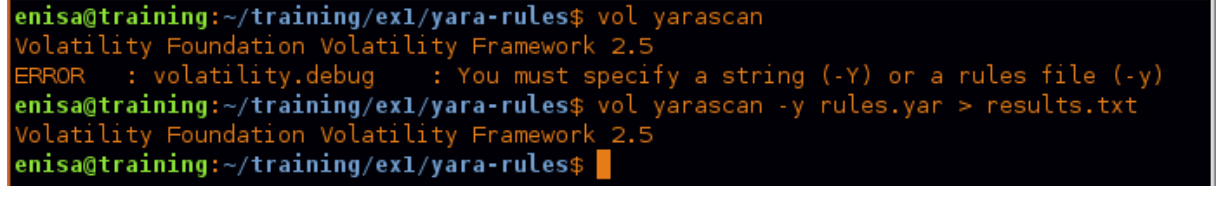
\includegraphics[width=0.8\textwidth]{fig-05.png}
\caption{\texttt{yarascan} results.}
\end{figure}
\begin{figure}[H]\centering
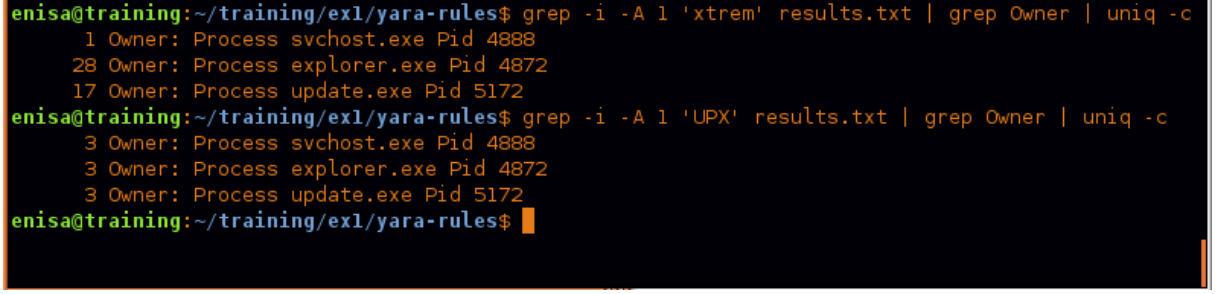
\includegraphics[width=0.8\textwidth]{fig-08.png}
\caption{Process listing (\texttt{pslist}).}
\end{figure}
\begin{figure}[H]\centering
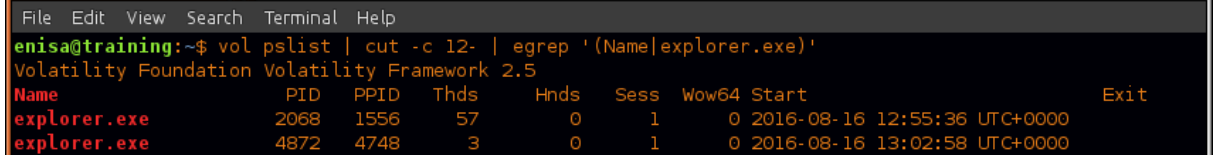
\includegraphics[width=0.8\textwidth]{fig-12.png}
\caption{Two \texttt{explorer.exe} processes (RunPE masquerade).}
\end{figure}

\subsection{Forensic Disk Image}
\textbf{Description:} Full disk image captured after the memory dump, mounted read-only.\\
\textbf{Collection / Review Method:} ClamAV scan; manual review of paths, timestamps, and browser cache/history.\\
\textbf{Relevant Facts Found:} CVE-2012-3993 exploit code in Firefox cache; \texttt{3568226350[1].exe} (Xtreme RAT) in INetCache; \texttt{\%TEMP\%\textbackslash svchost.exe}; \texttt{\%APPDATA\%\textbackslash HostData\textbackslash update.exe} confirmed Xtreme RAT; \texttt{EpUpdate} toolkit (13:14:47); \texttt{54948tp.exe} (13:10:03); history showing \texttt{blog.mycompany.ex} and the \texttt{blog.mysportclub.ex} download pattern; injected iframe.\\
\textbf{How It Supports the Investigation:} Confirms initial vector, payload delivery, staged toolkit; corroborates memory findings.\\
\textbf{Replication Steps:} Mount read-only; \texttt{clamscan -r}; enumerate Firefox \texttt{places.sqlite} and cache; inspect cached HTML for iframes; review \texttt{EpUpdate}/\texttt{\%TEMP\%} MAC times.

\begin{figure}[H]\centering
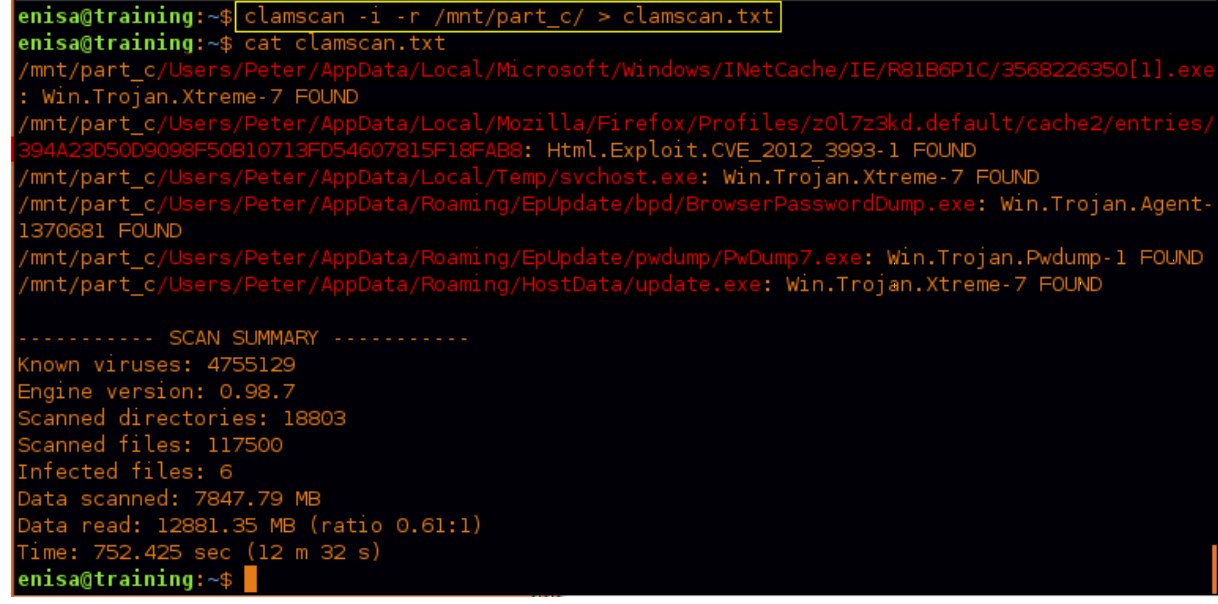
\includegraphics[width=0.8\textwidth]{fig-16.png}
\caption{ClamAV scan results.}
\end{figure}
\begin{figure}[H]\centering
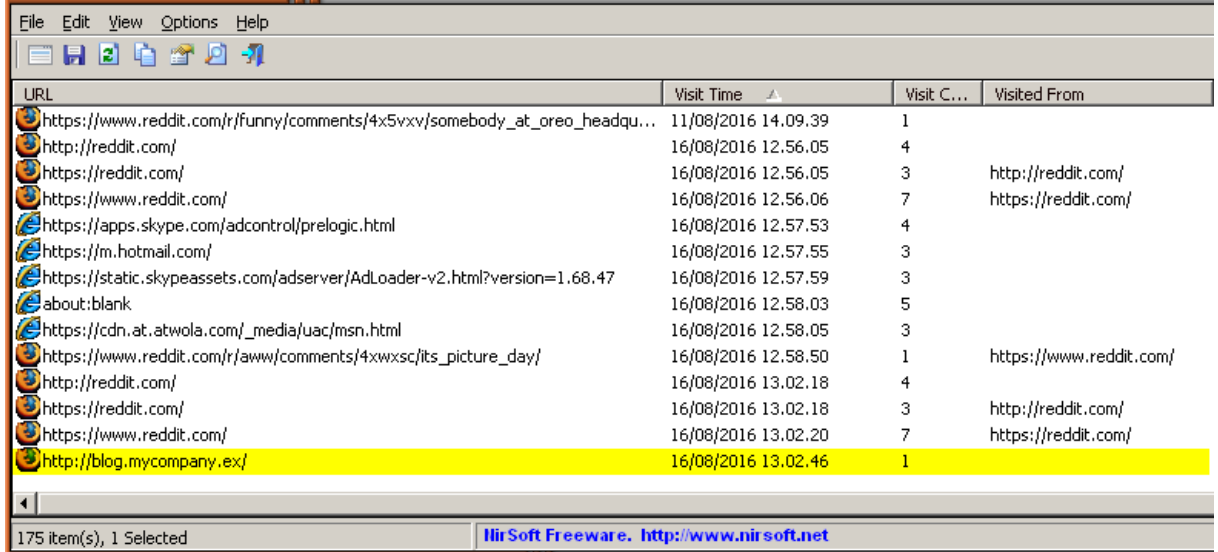
\includegraphics[width=0.8\textwidth]{fig-17.png}
\caption{Firefox browsing history.}
\end{figure}
\begin{figure}[H]\centering
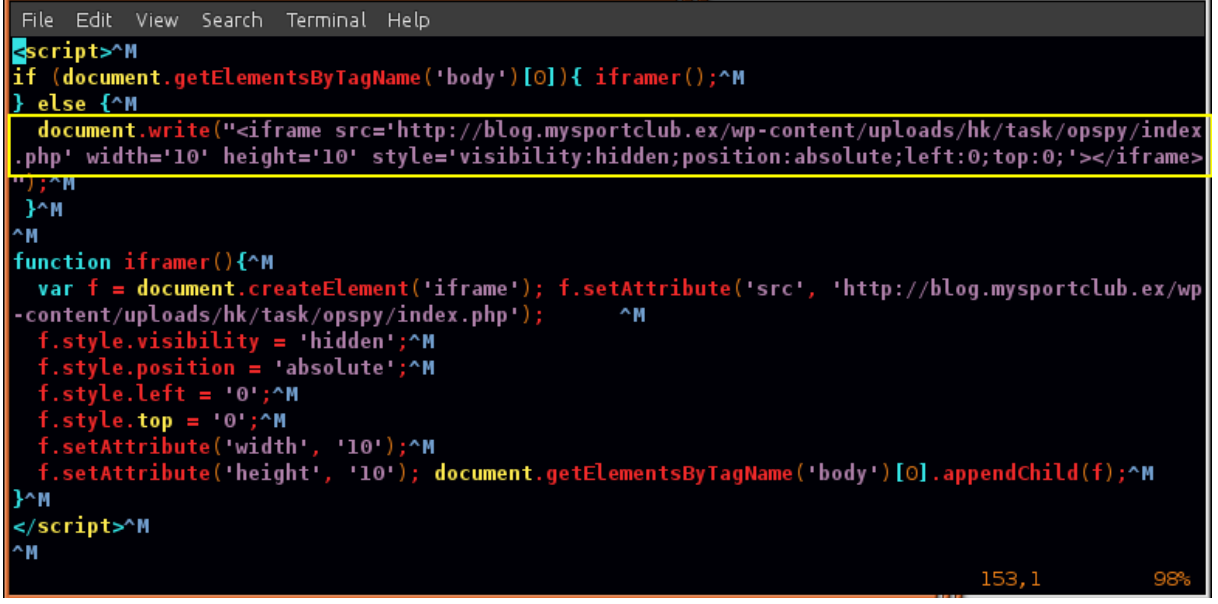
\includegraphics[width=0.8\textwidth]{fig-19.png}
\caption{Iframe injection to the Exploit Kit landing page.}
\end{figure}

\subsection{Payload / Downloader Analysis (\texttt{3568226350.exe}, \texttt{54948tp.exe})}
\textbf{Description:} PE32 executables built from Python via \texttt{py2exe}, recovered and decompiled.\\
\textbf{Collection / Review Method:} Static decompilation of embedded Python.\\
\textbf{Relevant Facts Found:} \texttt{DOWNLOAD\_URL} to \texttt{data\_32.bin} on \texttt{blog.mysportclub.ex}; \texttt{get\_toolz} downloads/decrypts/unpacks to \texttt{\%APPDATA\%\textbackslash EpUpdate}; \texttt{\%TMP\%\textbackslash SystemProfile} working dir; auto-run of mimikatz and BPD; \texttt{SystemProfile} held \texttt{bpd.log}, \texttt{mimikatz.log} (13:14:48), \texttt{sysinfo.txt} (13:34:25), \texttt{netscan/} (13:52:21) with Nmap XML for 192.168.5.1/.10/.15.\\
\textbf{How It Supports the Investigation:} Explains toolkit delivery; confirms credential-theft and reconnaissance objectives.\\
\textbf{Replication Steps:} Extract Python from the py2exe binary; decompile; review \texttt{DOWNLOAD\_URL}, \texttt{get\_toolz}, \texttt{main}; correlate \texttt{\%TMP\%\textbackslash SystemProfile} output.

\begin{figure}[H]\centering
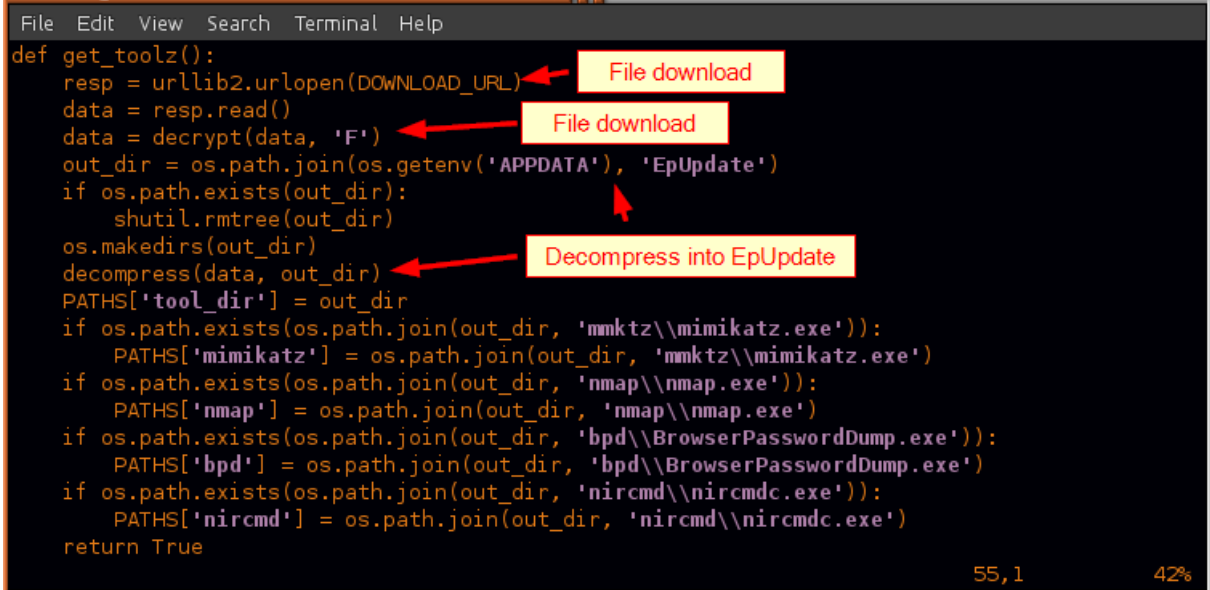
\includegraphics[width=0.8\textwidth]{fig-24.png}
\caption{\texttt{get\_toolz} download/unpack function.}
\end{figure}
\begin{figure}[H]\centering
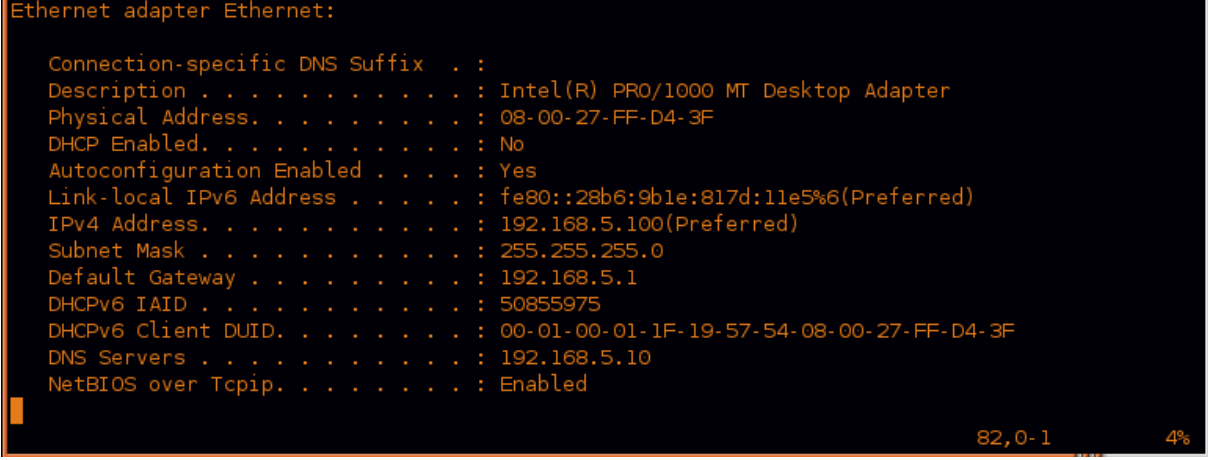
\includegraphics[width=0.8\textwidth]{fig-26.png}
\caption{Nmap scan output in \texttt{netscan/}.}
\end{figure}

\subsection{Prefetch}
\textbf{Description:} Windows Prefetch files documenting program execution.\\
\textbf{Collection / Review Method:} Prefetch parsing for names, run counts, last-run times.\\
\textbf{Relevant Facts Found:} \texttt{update.exe} 13:03:03--04; \texttt{54948tp.exe} 13:10:13; \texttt{mimikatz.exe}/\texttt{browserprocessdump.exe} 13:14:47; system-profiling 13:34:25--51 (and \texttt{whoami}/\texttt{ipconfig} 13:08--10); \texttt{nmap.exe} last 13:59:34 (earlier $\sim$13:56); \texttt{hydra.exe} 14:04:44; \texttt{plink.exe} six times (14:10:49--14:23:31); \texttt{pscp.exe} 14:47:12--14:50:09.\\
\textbf{How It Supports the Investigation:} Confirms dropped tools were executed; provides an attacker action timeline.\\
\textbf{Replication Steps:} Parse \texttt{C:\textbackslash Windows\textbackslash Prefetch\textbackslash *.pf}; sort by last-run; correlate with filesystem/registry timestamps.

\begin{figure}[H]\centering
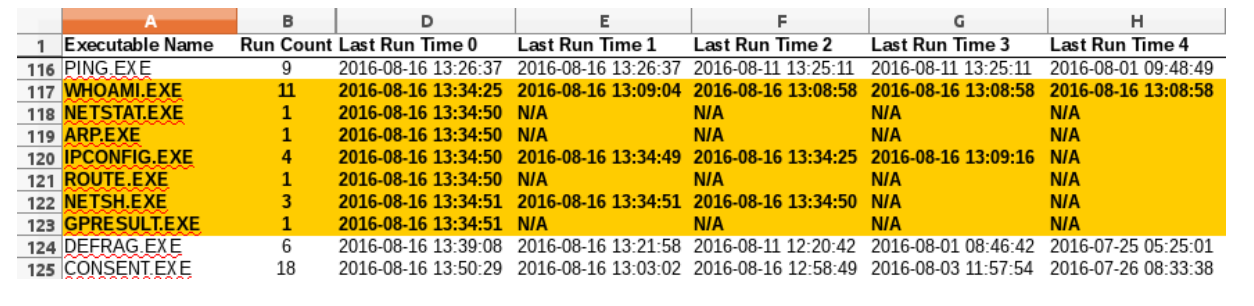
\includegraphics[width=0.8\textwidth]{fig-31.png}
\caption{\texttt{nmap.exe} and \texttt{hydra.exe} execution in Prefetch.}
\end{figure}

\subsection{Windows Event Logs}
\textbf{Description:} Security event logs around the Hydra window.\\
\textbf{Collection / Review Method:} Filtered query 14:03:00--14:05:00.\\
\textbf{Relevant Facts Found:} Three Event ID \textbf{4798} entries (14:02:04, 14:03:21, 14:04:43); two reference \texttt{hydra.exe} in EventData, matching the Prefetch Hydra time.\\
\textbf{How It Supports the Investigation:} Independently corroborates enumeration/credential-attack activity.\\
\textbf{Replication Steps:} Open Security log; filter Event ID 4798 for the window; inspect EventData for the process name.

\begin{figure}[H]\centering
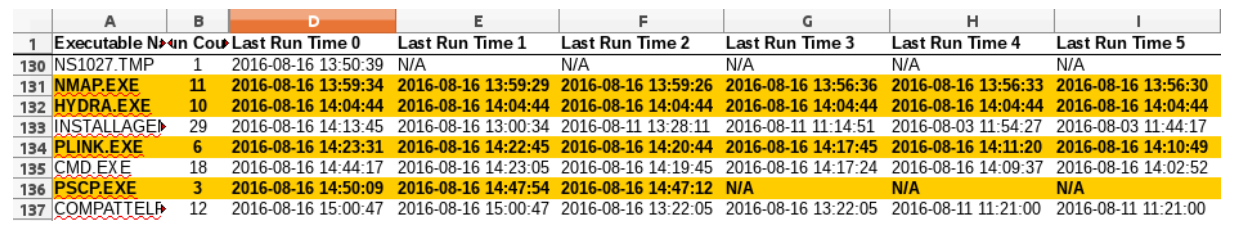
\includegraphics[width=0.8\textwidth]{fig-32.png}
\caption{Event 4798 entries related to \texttt{hydra.exe}.}
\end{figure}

\subsection{Registry (RegRipper / WRR)}
\textbf{Description:} \texttt{NTUSER.DAT} hive analysis.\\
\textbf{Collection / Review Method:} RegRipper \texttt{regtime} timeline; manual WRR inspection.\\
\textbf{Relevant Facts Found:} \texttt{Run}/\texttt{RunOnce} modified 13:02:57; \texttt{GhCtxq8t} created 13:03:10 (tied to \texttt{update.exe}, \texttt{FirstExecution} 13:03:10 UTC / 15:03:10 local); PuTTY keys modified 14:11:26; \texttt{SSHHostKeys} with RSA key for \textbf{192.168.5.10}; Uninstall data showing Firefox 33.0.3 and Adobe Flash 18.0.0.194.\\
\textbf{How It Supports the Investigation:} Confirms persistence, timezone offset, lateral movement to 192.168.5.10, and vulnerable software.\\
\textbf{Replication Steps:} Run RegRipper \texttt{regtime} on \texttt{NTUSER.DAT}; open in WRR; inspect \texttt{GhCtxq8t}, PuTTY \texttt{SSHHostKeys}, Uninstall subkeys.

\begin{figure}[H]\centering
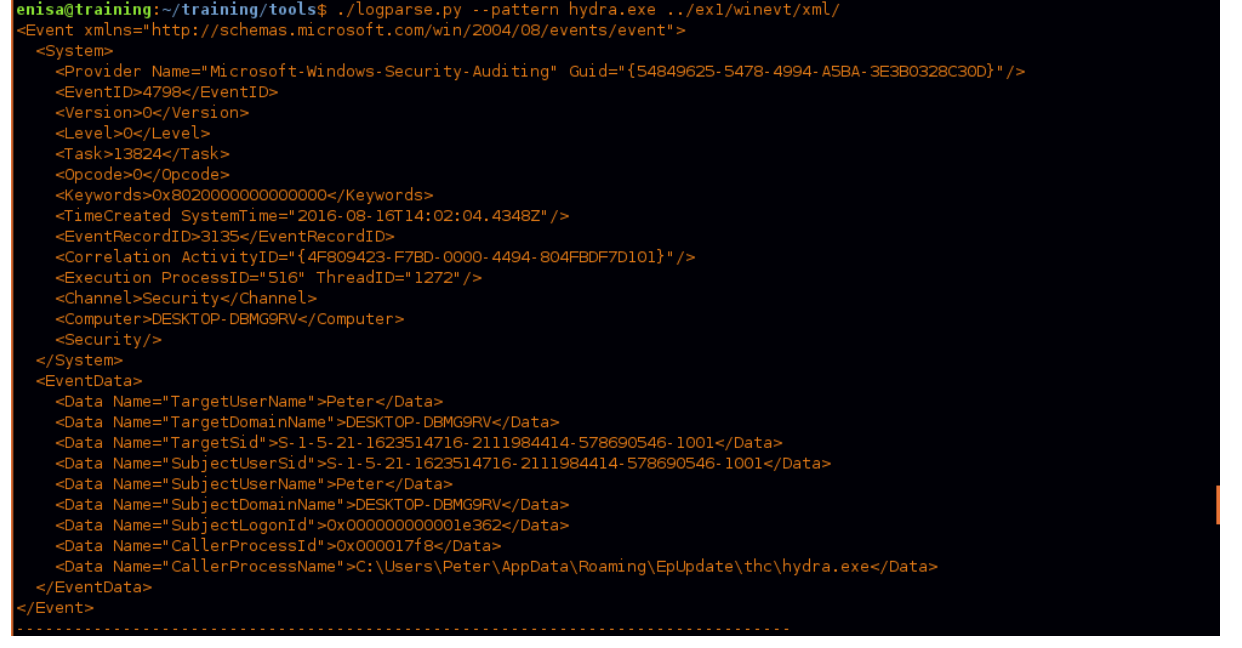
\includegraphics[width=0.8\textwidth]{fig-34.png}
\caption{\texttt{NTUSER.DAT} registry timeline (RegRipper).}
\end{figure}
\begin{figure}[H]\centering
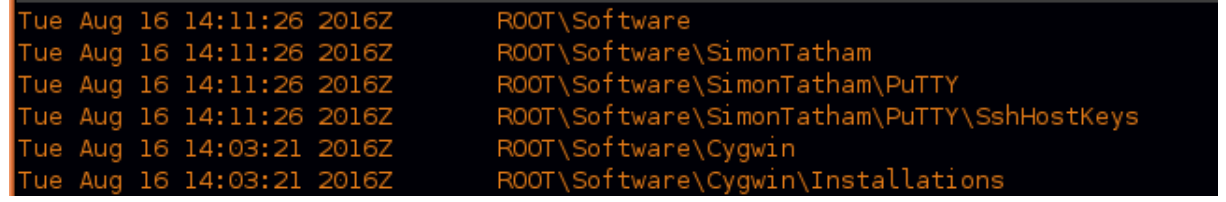
\includegraphics[width=0.8\textwidth]{fig-37.png}
\caption{\texttt{SSHHostKeys} with the RSA key for 192.168.5.10.}
\end{figure}

%============================ 8. REMEDIATION ============================
\section{Remediation}

\begin{itemize}
\item \textbf{Isolated the affected workstation} to stop any active attacker session (plink/pscp activity as late as 14:50 UTC).
\item \textbf{Reset the compromised user credentials} and, given mimikatz/Pwdump/BrowserPasswordDump and the \texttt{wdigest.reg} (\texttt{UseLogonCredential}) change, reset credentials for any account that logged into the host, prioritizing privileged accounts.
\item \textbf{Reverted the WDigest change}, restoring \texttt{UseLogonCredential} to 0 to stop cleartext credential caching.
\item \textbf{Removed malicious files}: \texttt{\%APPDATA\%\textbackslash HostData\textbackslash update.exe}, \texttt{\%TEMP\%\textbackslash svchost.exe}, \texttt{\%TEMP\%\textbackslash 54948tp.exe}, \texttt{\%TEMP\%\textbackslash 3568226350.exe}, \texttt{\%APPDATA\%\textbackslash EpUpdate\textbackslash}, and \texttt{\%TMP\%\textbackslash SystemProfile\textbackslash}.
\item \textbf{Removed persistence} by deleting \texttt{GhCtxq8t} and cleaning malicious \texttt{Run}/\texttt{RunOnce} entries.
\item \textbf{Blocked attacker infrastructure}: domains \texttt{blog.mycompany.ex} and \texttt{blog.mysportclub.ex} and IP 151.80.137.2.
\item \textbf{Reimaged the workstation} from a known-good build given the depth of compromise.
\item \textbf{Investigated internal host 192.168.5.10} (SSH host key recorded; plink target) and reviewed 192.168.5.1 and 192.168.5.15.
\item \textbf{Verified no additional IOC hits} on other endpoints and \textbf{increased monitoring} (DNS, proxy, endpoint) after containment.
\end{itemize}

%============================ 9. RECOMMENDATIONS ============================
\section{Recommendations}

\subsection{Short-Term Recommendations}
\begin{itemize}
\item Patch or remove the exploited software --- upgrade Firefox from 33.0.3 and remove/update the end-of-life Adobe Flash plugin (18.0.0.194).
\item Reset affected passwords for the user and any account exposed on the host; force a domain-wide reset of privileged credentials.
\item Block the Section~6 IOCs at the perimeter and add file/registry indicators to endpoint detection.
\item Reimage the affected host and remove \texttt{GhCtxq8t} persistence and dropped tooling (performed; verify on rebuild).
\item Sweep peer workstations for the same IOCs, especially any that browsed the attacker domains.
\item Examine internal host 192.168.5.10 for successful lateral movement.
\end{itemize}

\subsection{Long-Term Recommendations}
\begin{itemize}
\item Implement vulnerability and patch management focused on browsers and plugins; retire legacy plugins such as Flash.
\item Deploy EDR to detect RAT behavior, RunPE masquerading, and credential dumpers like mimikatz.
\item Centralize logs in a SIEM (Windows Security, PowerShell, proxy, DNS) to enable correlation like the Event 4798 / Hydra timeline.
\item Enforce least privilege so a single workstation compromise cannot readily reach internal hosts or store cleartext credentials.
\item Implement web filtering / DNS security to block Exploit-Kit domains proactively.
\item Establish regular threat hunting using the documented IOC and behavioral patterns.
\item Deliver user awareness training and maintain an incident response playbook for drive-by/RAT scenarios.
\end{itemize}

%============================ 10. LESSONS LEARNED ============================
\section{Lessons Learned}

This investigation reinforced the value of building a single, correlated timeline from independent evidence sources. Memory analysis identified the malware family and masquerade technique; the disk image and browser artifacts revealed the initial vector; Prefetch confirmed which tools actually executed; Event Logs and the registry corroborated the timing of credential attacks, persistence, and lateral movement. No single artifact told the whole story, but together they produced a coherent Who/What/When/Where/Why/How narrative, and investigative leads converted quickly into actionable IOCs suitable for enterprise-wide hunting.

The engagement also highlighted the operational importance of disciplined evidence handling and repeatable procedures: documenting the Volatility profile and offsets, the ClamAV scan method, and the Prefetch/registry parsing steps means a third party can reproduce every conclusion. Going forward, the team will continue to prioritize timeline correlation, keep reports concise for executive readers while confining deep technical detail to the evidence and appendix sections, and preserve original images so findings remain defensible.

%============================ 11. APPENDICES ============================
\section{Appendices}

\subsection*{Appendix A: Key Artifact Timestamps (UTC)}
\begin{itemize}
\item 12:54:24 --- System boot
\item 13:02:46 --- Visit to \texttt{blog.mycompany.ex}
\item 13:02:57 --- \texttt{svchost.exe} created in \texttt{\%TEMP\%}; \texttt{Run}/\texttt{RunOnce} modified
\item 13:03:04 --- \texttt{update.exe} executed
\item 13:03:10 --- \texttt{GhCtxq8t} persistence created (first execution)
\item 13:10:03 / 13:10:13 --- \texttt{54948tp.exe} created / executed
\item 13:14:47 --- \texttt{EpUpdate} toolkit created
\item 13:34:25--13:34:51 --- Local system profiling
\item 13:59:xx --- Nmap scans of 192.168.5.1/.10/.15
\item 14:04:44 --- Hydra executed
\item 14:10:49--14:23:31 --- \texttt{plink.exe} (six executions)
\item 14:47:12--14:50:09 --- \texttt{pscp.exe} (three executions)
\end{itemize}

\subsection*{Appendix B: \texttt{\%APPDATA\%\textbackslash EpUpdate} Toolkit Contents}
\texttt{bpd/} (BrowserPasswordDump.exe), \texttt{mmktz/} (mimikatz), \texttt{nircmd/} (NirCmd), \texttt{nmap/} (Nmap 7.12), \texttt{pwdump/} (Pwdump), \texttt{ssh/} (plink, pscp), \texttt{thc/} (THC Hydra), \texttt{passwords.txt} (common-password list), \texttt{wdigest.reg} (sets \texttt{UseLogonCredential}).

\subsection*{Appendix C: Consolidated Attack Timeline Figures}
\begin{figure}[H]\centering
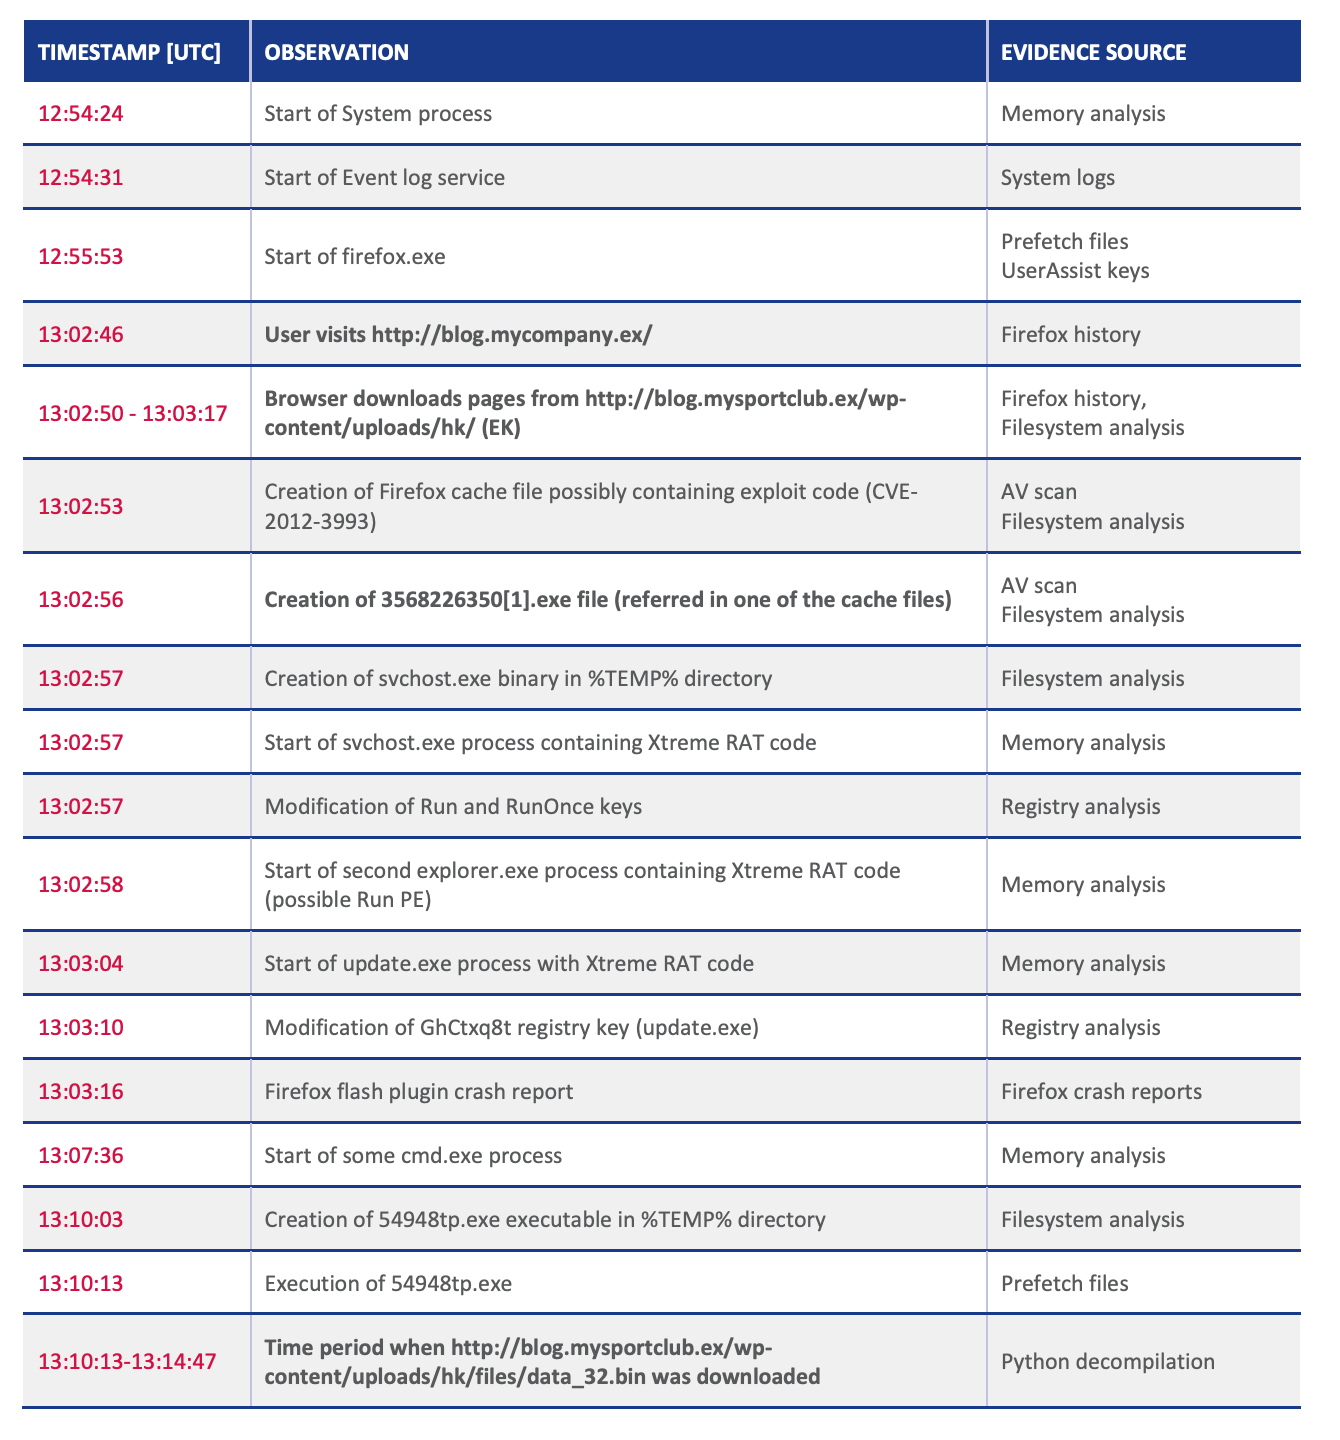
\includegraphics[width=0.85\textwidth]{fig-41.png}
\caption{Overall event timeline --- part 1.}
\end{figure}
\begin{figure}[H]\centering
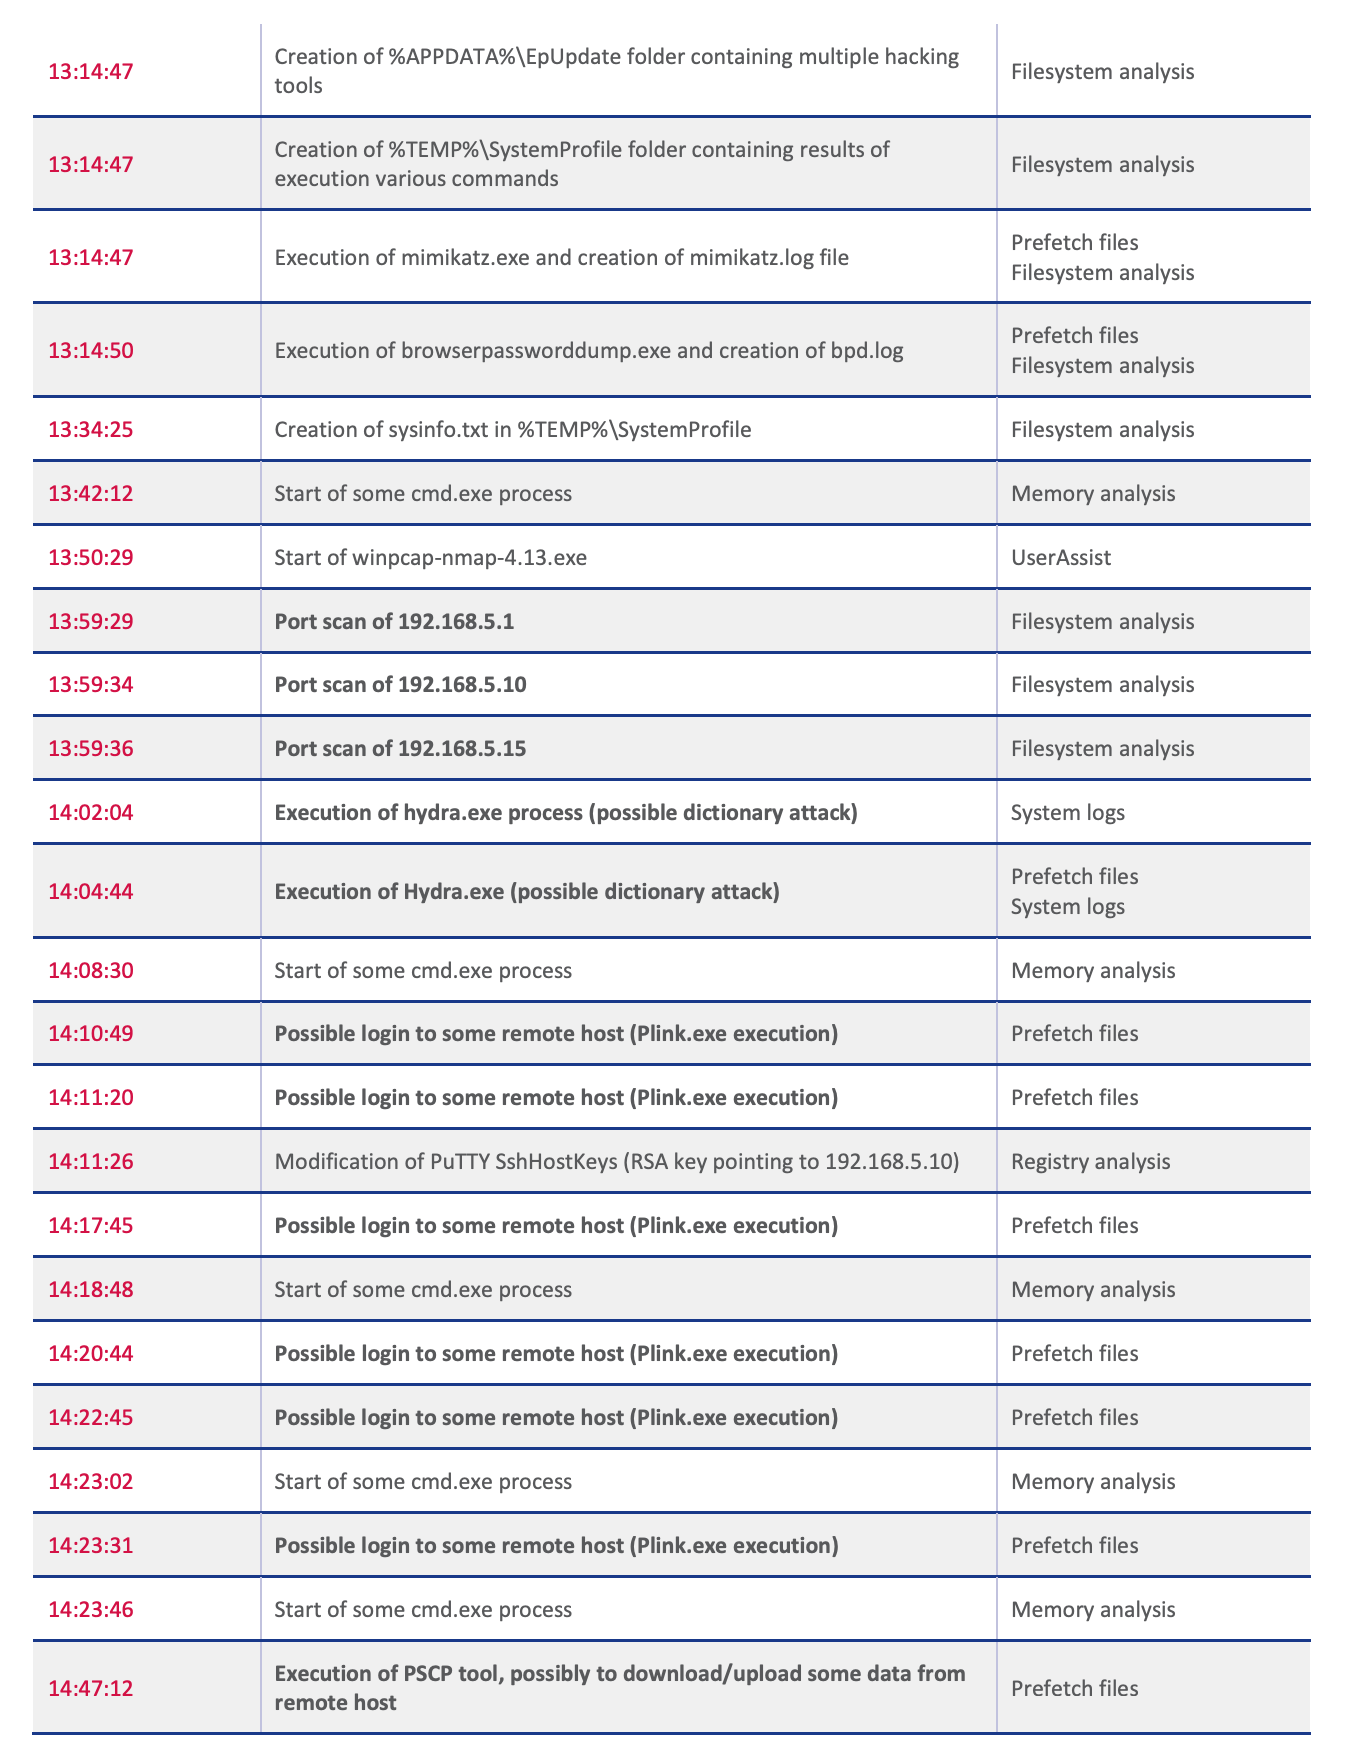
\includegraphics[width=0.85\textwidth]{fig-42.png}
\caption{Overall event timeline --- part 2.}
\end{figure}
\begin{figure}[H]\centering
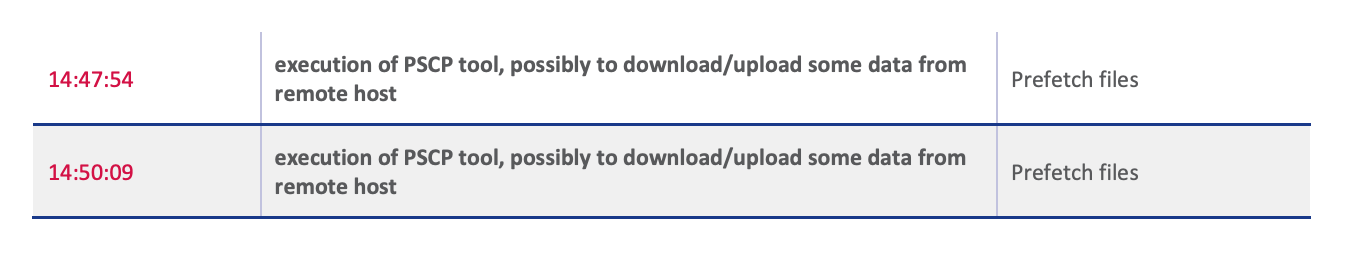
\includegraphics[width=0.85\textwidth]{fig-43.png}
\caption{Overall event timeline --- part 3.}
\end{figure}

\subsection*{Appendix D: Additional Supporting Screenshots}
\begin{figure}[H]\centering
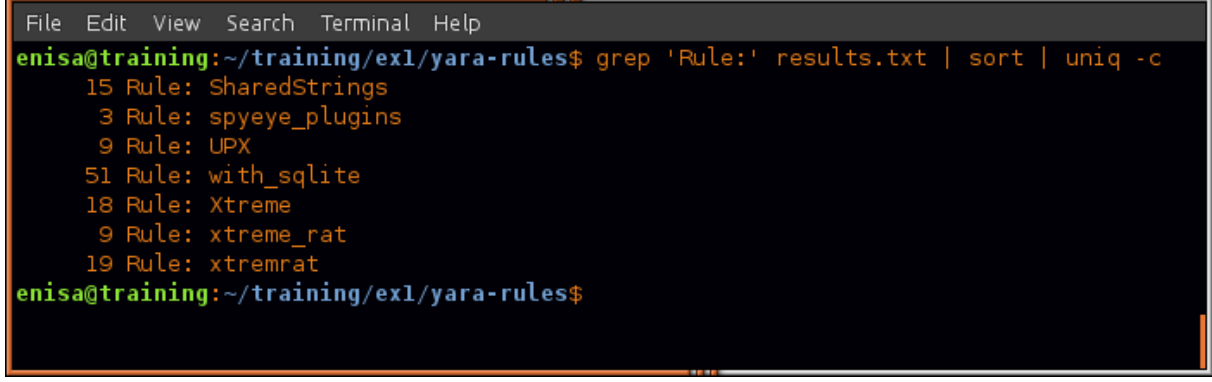
\includegraphics[width=0.75\textwidth]{fig-07.png}
\caption{Processes with Xtreme RAT / UPX-packed code.}
\end{figure}
\begin{figure}[H]\centering
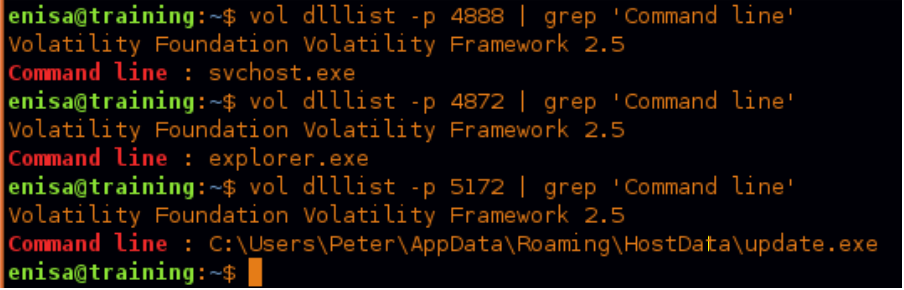
\includegraphics[width=0.75\textwidth]{fig-11.png}
\caption{Command line used to start each process (\texttt{dlllist}).}
\end{figure}
\begin{figure}[H]\centering
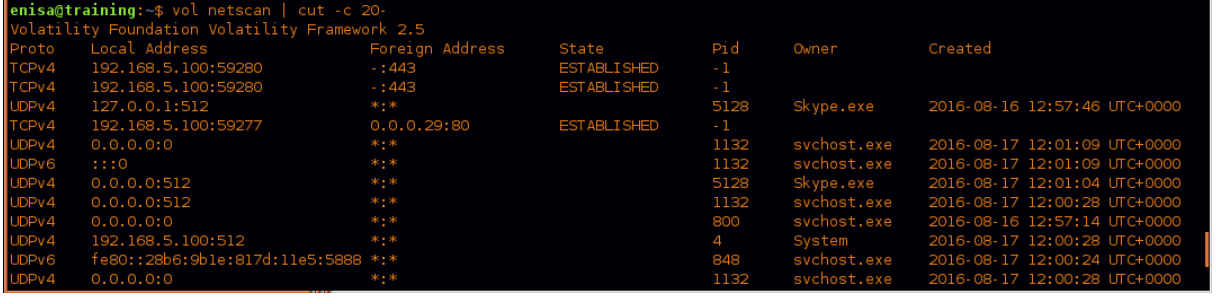
\includegraphics[width=0.75\textwidth]{fig-13.png}
\caption{Network connections (\texttt{netscan}).}
\end{figure}
\begin{figure}[H]\centering
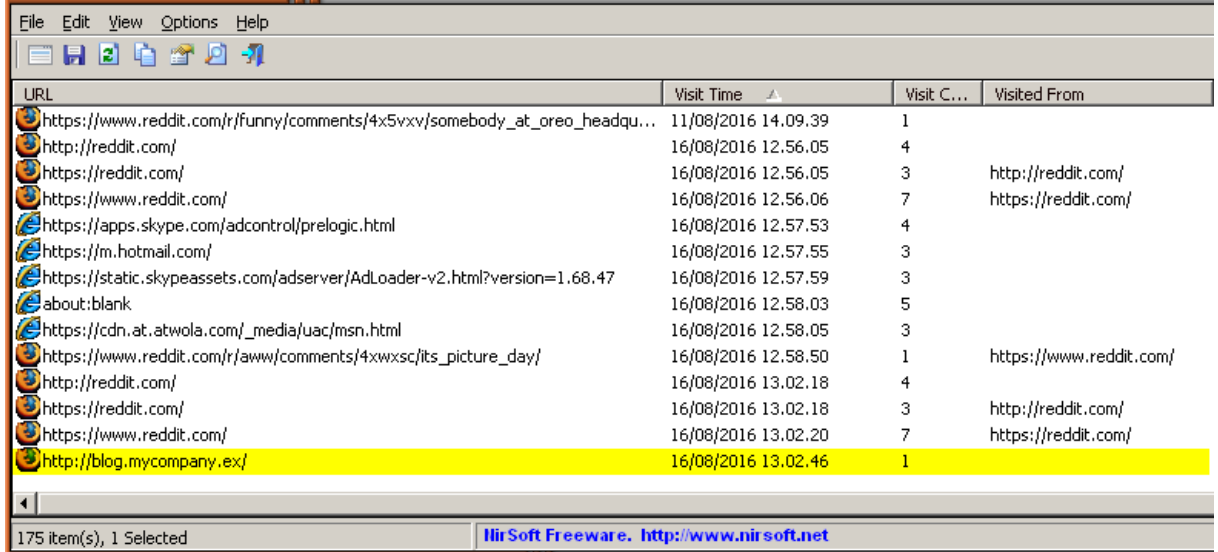
\includegraphics[width=0.75\textwidth]{fig-18.png}
\caption{Suspicious script invoked in \texttt{blog.mycompany.ex.htm}.}
\end{figure}
\begin{figure}[H]\centering
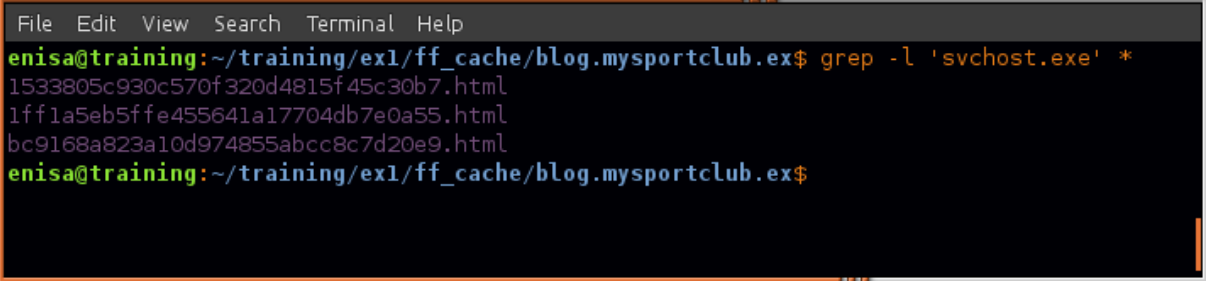
\includegraphics[width=0.75\textwidth]{fig-21.png}
\caption{Code that downloads and executes \texttt{3568226350.exe}.}
\end{figure}
\begin{figure}[H]\centering
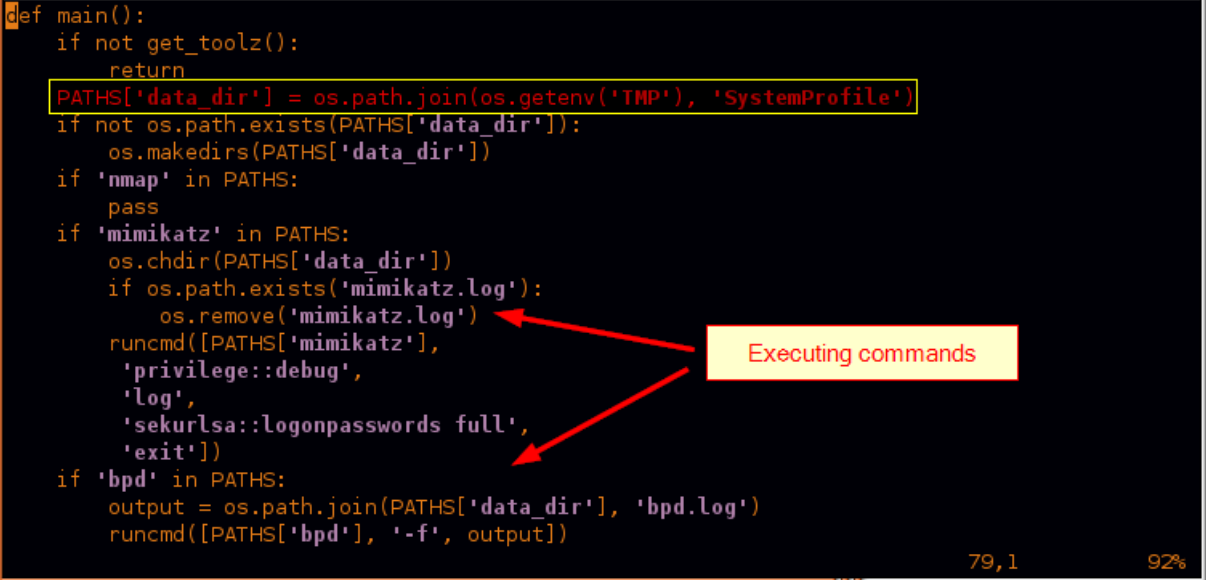
\includegraphics[width=0.75\textwidth]{fig-25.png}
\caption{Contents of \texttt{\%TMP\%\textbackslash SystemProfile}.}
\end{figure}
\begin{figure}[H]\centering
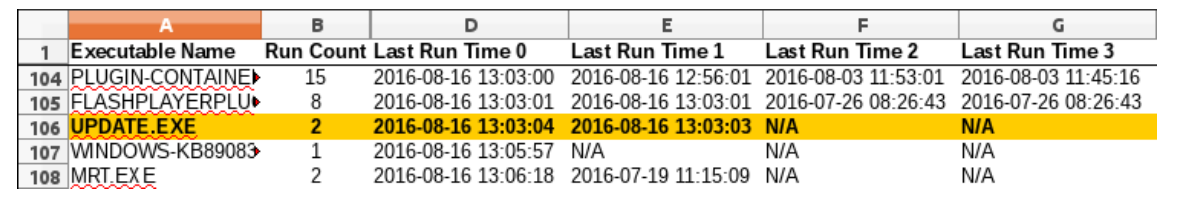
\includegraphics[width=0.75\textwidth]{fig-29.png}
\caption{Execution of \texttt{54948tp.exe}, \texttt{mimikatz.exe}, and \texttt{browserprocessdump.exe}.}
\end{figure}
\begin{figure}[H]\centering
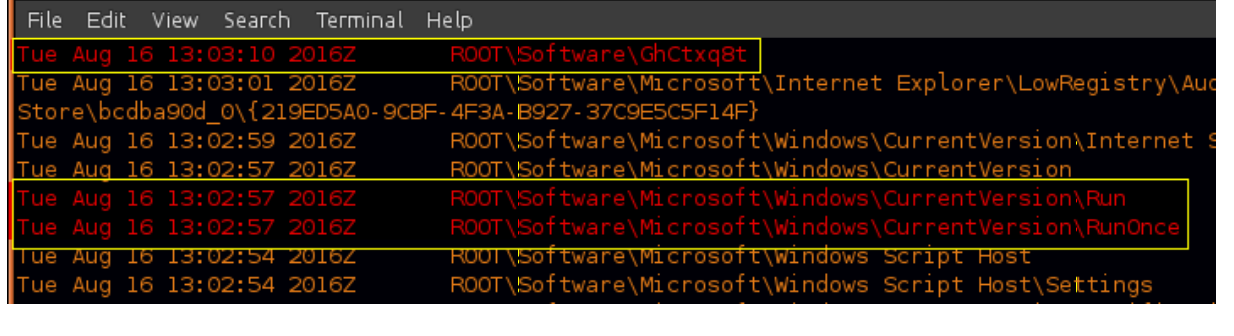
\includegraphics[width=0.75\textwidth]{fig-35.png}
\caption{\texttt{GhCtxq8t} subkey associated with \texttt{update.exe} (WRR).}
\end{figure}
\begin{figure}[H]\centering
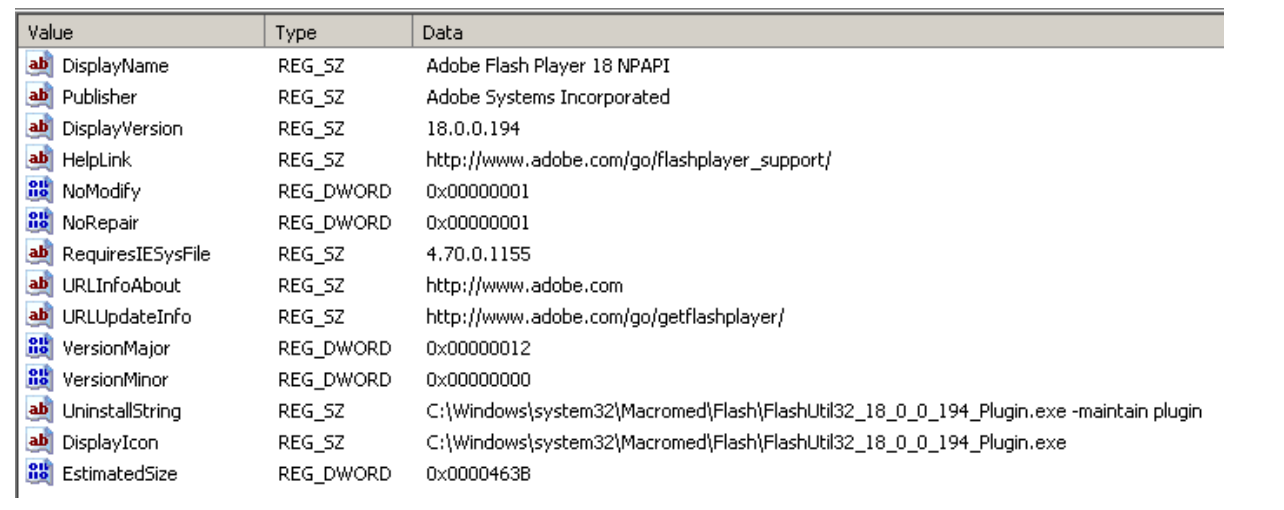
\includegraphics[width=0.75\textwidth]{fig-39.png}
\caption{Outdated Mozilla Firefox 33.0.3.}
\end{figure}
\begin{figure}[H]\centering
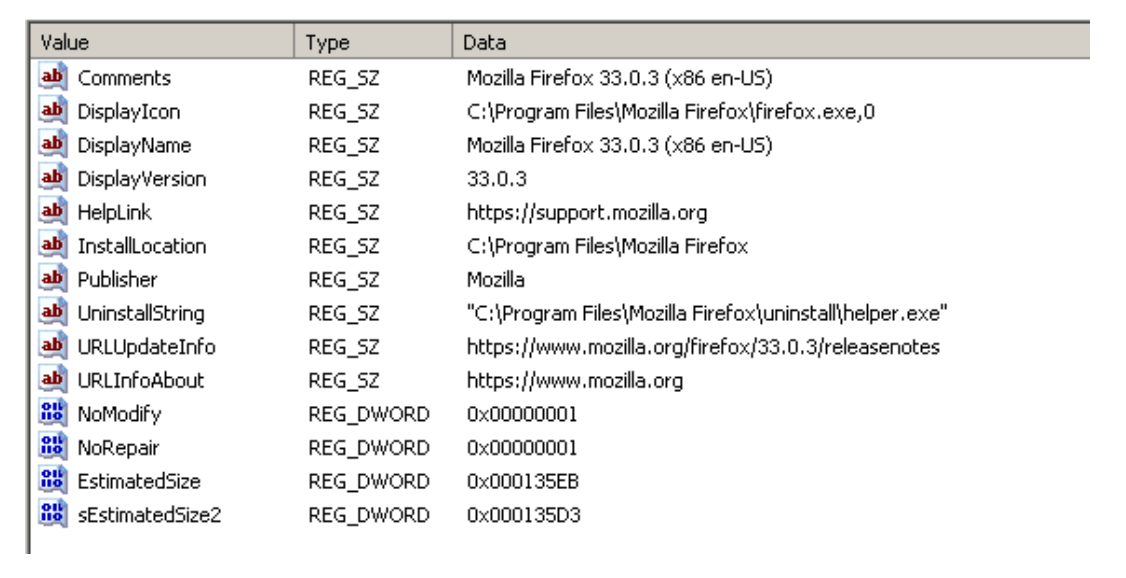
\includegraphics[width=0.75\textwidth]{fig-40.png}
\caption{Outdated Adobe Flash Plugin 18.0.0.194.}
\end{figure}

%============================ 12. REFERENCES ============================
\section{References}

No external sources were used. This report was prepared from the provided evidence document and its supporting figures.

\end{document}
